\documentclass[12pt]{article}
\usepackage[utf8]{inputenc}

\usepackage{lmodern}

\usepackage{enumitem}
\usepackage[margin=2cm]{geometry}

\usepackage{amsmath, amsfonts, amssymb}
\usepackage{graphicx}
%\usepackage{subfigure}
\usepackage{tikz}
\usepackage{pgfplots}
\usepackage{multicol}

\usepackage{comment}
\usepackage{url}
\usepackage{calc}
\usepackage{subcaption}
\usepackage[indent=0pt]{parskip}
\usepackage{animate}

\usepackage{array}
\usepackage{blkarray,booktabs, bigstrut}
\usepackage{bigints}

\pgfplotsset{compat=1.16}

% MATH commands
\newcommand{\ga}{\left\langle}
\newcommand{\da}{\right\rangle}
\newcommand{\oa}{\left\lbrace}
\newcommand{\fa}{\right\rbrace}
\newcommand{\oc}{\left[}
\newcommand{\fc}{\right]}
\newcommand{\op}{\left(}
\newcommand{\fp}{\right)}

\newcommand{\bi}{\mathbf{i}}
\newcommand{\bj}{\mathbf{j}}
\newcommand{\bk}{\mathbf{k}}
\newcommand{\bF}{\mathbf{F}}

\newcommand{\mR}{\mathbb{R}}

\newcommand{\ra}{\rightarrow}
\newcommand{\Ra}{\Rightarrow}

\newcommand{\sech}{\mathrm{sech}\,}
\newcommand{\csch}{\mathrm{csch}\,}
\newcommand{\curl}{\mathrm{curl}\,}
\newcommand{\dive}{\mathrm{div}\,}

\newcommand{\ve}{\varepsilon}
\newcommand{\spc}{\vspace*{0.5cm}}

\DeclareMathOperator{\Ran}{Ran}
\DeclareMathOperator{\Dom}{Dom}

\newcommand{\exo}[1]{\noindent\textcolor{red}{\fbox{\textbf{Problem {#1}}}\hrulefill}\\}
\newcommand{\qu}[4]{\noindent\textcolor{#4}{\fbox{\textbf{Section {#1} | Problem {#2}}} \hrulefill{{\fbox{\textbf{{#3} Points}}}}\\}}

\newcommand{\semester}{Spring 2023}

\newcommand{\CVup}{%

\begin{tikzpicture}
\draw[black, <->, >=latex] (-0.33, 0.5) .. controls (-0.125, 0) and (0.125, 0) .. (0.33, 0.5);
\end{tikzpicture}}

\newcommand{\CVupInc}{%
\begin{tikzpicture}
\draw[black, ->, >=latex] (0,0) .. controls (0.2, 0) and (0.4, 0.2) .. (0.5, 0.5);
\end{tikzpicture}}

\newcommand{\CVupDec}{%
\begin{tikzpicture}[rotate=270]
\draw[black, ->, >=latex] (0,0) .. controls (0.2, 0) and (0.4, 0.2) .. (0.5, 0.5);
\end{tikzpicture}}

\newcommand{\CVdown}{%
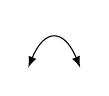
\begin{tikzpicture}
\draw[black, <->, >=latex] (-0.33, -0.5) .. controls (-0.125, 0) and (0.125, 0) .. (0.33, -0.5);
\end{tikzpicture}}

\newcommand{\CVdownInc}{%
\begin{tikzpicture}
\draw[black, ->, >=latex] (-0.5, -0.5) .. controls (-0.5, -0.3) and (-0.5, -0.1) .. (0,0);
\end{tikzpicture}}

\newcommand{\CVdownDec}{%
\begin{tikzpicture}[rotate=-90]
\draw[black, ->, >=latex] (-0.5, -0.5) .. controls (-0.5, -0.3) and (-0.5, -0.1) .. (0,0);
\end{tikzpicture}}

\begin{document}
	\noindent \hrulefill \\
	MATH-241 \hfill Pierre-Olivier Paris{\'e}\\
	Solutions Section 2-1 \hfill \semester \\\vspace*{-1cm}
	
	\noindent\hrulefill
	
	\spc
	
	\exo{5}
	\\
	The equation of the tangent line at the point $(x_0 , y_0 ) = (2, -4)$ is
		\begin{align*}
		y + 4 = m (x - 2)
		\end{align*}
	where $m = f'(2)$. The derivative is given by the limit of the different quotient:
		\begin{align*}
		\frac{f (2 + h) - f(2)}{h} & = \frac{4(2 + h) - 3(2 + h)^2 + 4}{h} \\
		&= \frac{8 + 4h - 3(4 + 4h + h^2) + 4}{h} \\
		&= \frac{-4 - 8h - 3h^2 + 4}{h} \\
		&= -8 - 3h
		\end{align*}
	and as $h \ra 0$, we get $f'(2) = -8$. So, we get
		\begin{align*}
		y + 4 = -8 (x - 2) .
		\end{align*}
		
	\spc
	
	\exo{6}
	\\
	The equation of the tangent line at $(2, 3)$ is 
		\begin{align*}
		y - 3 = f'(2) (x - 2) .
		\end{align*}
	We have to find $f'(2)$. We have $f(x) = x^3 - 3x + 1$, and therefore
		\begin{align*}
		f' (2) = \lim_{h \ra 0} \frac{f (2 + h) - f(2)}{h} &= \lim_{h \ra 0} \frac{ (2 + h)^3 - 3(2 + h) + 1 - 3}{h} \\
		&= \lim_{h \ra 0} \frac{8 + 12h + 6h^2 + h^3 - 6 - 3h + 1 - 3}{h} \\
		&= \lim_{h \ra 0} \frac{9h + 2h^2 + h^3}{h} \\
		&= \lim_{h \ra 0} 9 + 2h + h^2 \\
		&= 9 .
		\end{align*}
	Therefore, we obtain $f' (2) = 9$. Therefore, the equation of the tangent line is	
		\begin{align*}
		y = 9x - 18 + 3 = 9x - 15 .
		\end{align*}
	
	\spc
	
	\exo{34}
	\\
	The value of $f'(a)$ is given by
		\begin{align*}
		f' (a) = \lim_{h \ra 0} \frac{f (a + h) - f(a)}{h} .
		\end{align*}
	Evaluating $f$ at $a + h$ and at $a$ in this expression, we can do some calculations:
		\begin{align*}
		\lim_{h \ra 0} \frac{f (a + h) - f(a)}{h} &= \lim_{h \ra 0} \frac{\frac{1}{(a + h)^2} - \frac{1}{a^2}}{h} \\
		&= \lim_{h \ra 0} \frac{a^2 - (a + h)^2}{(a + h)^2 a^2 h} \\
		&= \lim_{h \ra 0} \frac{a^2 - a^2 - 2ah - h^2}{(a + h)^2 a^2 h} \\
		&= \lim_{h \ra 0} -\frac{2ah + h^2}{(a + h)^2 a^2 h} \\
		&= \lim_{h \ra 0} - \frac{2a + h}{(a + h)^2 a^2} \\
		&= -\frac{2a}{a^4} \\
		&= -\frac{2}{a^3} .
		\end{align*}
	Therefore, we get $f'(a) = -2/a^3$. 
	
	\spc
	
	\exo{44}
	\\
	The velocity at $t = 4$ is given by $f'(4)$. This is given by
		\begin{align*}
		\lim_{h \ra 0} \frac{f(4 + h) - f(4)}{h} &= \lim_{h \ra 0} \frac{10 + \frac{45}{5 + h} - 10 - \frac{45}{5}}{h} \\
		&= \lim_{h \ra 0} \frac{\frac{45}{5 + h} - 9}{h} \\
		&= \lim_{h \ra 0} \frac{45 - 45 - 9h}{(5 + h) h} \\
		&= \lim_{h \ra 0} - \frac{9h}{(5 + h) h} \\
		&= \lim_{h \ra 0} -\frac{9}{5+ h} .
		\end{align*}
	Evaluating the last limit with the Quotient Rule, we get $f' (4) = -9/5$. 
	
	\newpage
	
	\exo{60}
	\\
	By definition, we have
		\begin{align*}
		f' (0) &= \lim_{h \ra 0} \frac{f (0 + h) - f(0)}{h} \\
		&= \lim_{h \ra 0} \frac{h^2 \sin (1/h)}{h} \\
		&= \lim_{h \ra 0} h \sin (1/h ) .
		\end{align*}
	The last limit exists because
		\begin{align*}
		-h \leq h \sin (1/h ) \leq h
		\end{align*}
	for any $h > 0$ and
		\begin{align*}
		h \leq h \sin (1/h) \leq -h
		\end{align*}
	when $h < 0$. We can simplify this by using the absolute value:
		\begin{align*}
		0 \leq |h \sin (1/h)| \leq |h|
		\end{align*}
	because $0 \leq |\sin (1/h)| \leq 1$. Using the Squeeze Theorem, we conclude that
		\begin{align*}
		\lim_{h \ra 0} h \sin (1/h) = 0 .
		\end{align*}
	Therefore, $f'(0)$ exists and $f'(0) = 0$.
	
	
\end{document}